\documentclass[11pt]{article}

\usepackage[T1]{fontenc}
\usepackage[utf8]{inputenc}
\usepackage{newtxtext,newtxmath}
\usepackage[margin=0.8in]{geometry}
\usepackage{graphicx}
\usepackage{float}
\usepackage{booktabs}
\usepackage{array}
\usepackage{siunitx}
\usepackage{setspace}
\usepackage[font=small,labelfont=bf]{caption}
\usepackage[colorlinks,urlcolor=blue,linkcolor=black]{hyperref}

\graphicspath{{figures/}}
\setstretch{1.08}
\emergencystretch=2em

\title{Supporting Information for\\
Local-environment-dependent transferability of a fine-tuned MACE potential for
lithium adsorption on graphene defects}
\author{Yuhan Sun and Xiao Huang$^*$}
\date{}

\begin{document}
\maketitle

\begin{center}
$^*$Corresponding author: Xiao Huang (Xiao.huang@duke.edu)\\
Yuhan Sun and Xiao Huang contributed equally to this work.
\end{center}

\section{Dataset composition and MACE evaluation details}

The DFT label set contains 273 configurations: 194 ionic-relaxation frames and
79 fixed-geometry site or interpolation-path frames. The original
same-workflow split contains 211 training, 31 validation, and 31 test frames.
Because images from a shared interpolation path can appear in multiple
partitions, this split is used only to quantify interpolation within the sampled
workflow. The grouped split keeps each path intact and contains 263 training,
5 validation, and 5 test frames. Each grouped validation and test partition
contains one configuration from each structural family.

\begin{figure}[H]
  \centering
  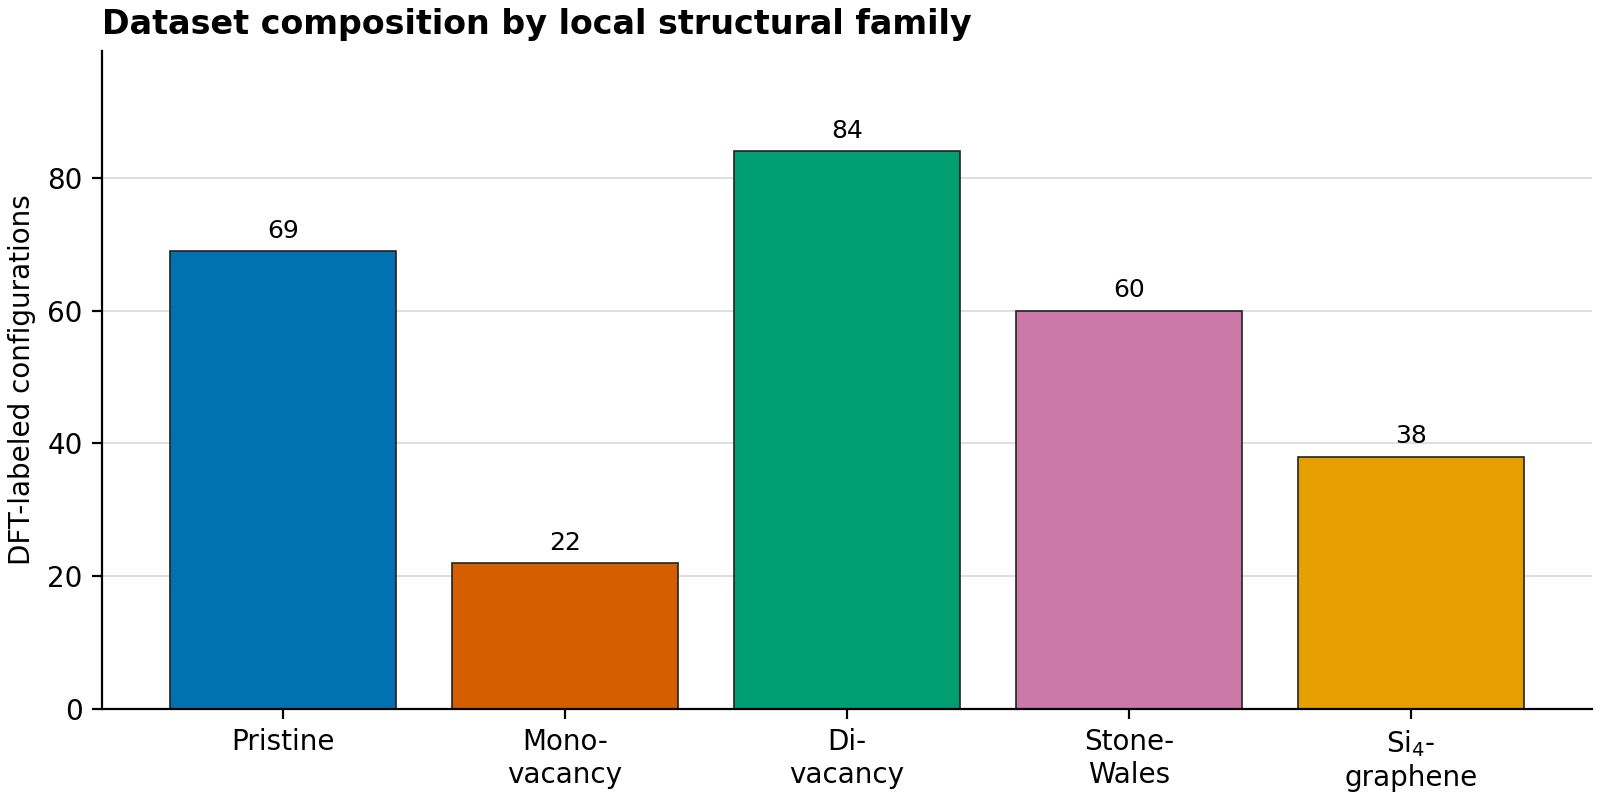
\includegraphics[width=0.72\textwidth]{dataset_family_counts.png}
  \caption{Number of DFT-labeled configurations in each structural family.}
  \label{fig:si_dataset_counts}
\end{figure}

\begin{table}[H]
  \centering
  \caption{External evaluator results on the original same-workflow split.
  Energy RMSE is in meV atom$^{-1}$ and force RMSE is the frame-level RMS
  force error in meV \AA$^{-1}$.}
  \label{tab:si_mace_errors}
  \begin{tabular}{lcc}
    \toprule
    Model and split or family & Energy RMSE & Force RMSE \\
    \midrule
    Foundation, test all & 50.0 & 285.2 \\
    Fine-tuned, training all & 41.2 & 10.3 \\
    Fine-tuned, validation all & 39.2 & 39.0 \\
    Fine-tuned, test all & 39.1 & 20.1 \\
    Fine-tuned test: pristine graphene & 5.3 & 12.7 \\
    Fine-tuned test: monovacancy graphene & 5.2 & 16.3 \\
    Fine-tuned test: divacancy graphene & 2.8 & 29.3 \\
    Fine-tuned test: Stone--Wales graphene & 3.5 & 19.3 \\
    Fine-tuned test: Si$_4$--graphene motif & 108.3 & 6.8 \\
    \bottomrule
  \end{tabular}
\end{table}

The first-stage grouped-$E_0$ checkpoint gives force RMSEs of 19.6, 10.9,
13.7, 42.9, and 9.2 meV \AA$^{-1}$ for the single grouped test configurations
from pristine, monovacancy, divacancy, Stone--Wales, and Si$_4$--graphene,
respectively. These one-frame family values are not population error estimates.
The three additional fine-tuning seeds give internal validation force metrics
of 96.4, 107.2, and 48.4 meV \AA$^{-1}$ in the archived MACE logs. These internal
metrics are not combined with the external frame-RMS values in
Table~\ref{tab:si_mace_errors}.

Foundation-assisted $E_0$ estimation was performed over all 263 grouped
training configurations. The archived fit has full elemental rank (3/3) and
gives baseline corrections of -3.271318, -1.246324, and -1.280346 eV for Li,
C, and Si, respectively. These quantities are model baseline corrections, not
isolated-atom energies.

\begin{table}[H]
  \centering
  \footnotesize
  \caption{Relationship between a representative concurrent-learning workflow
  and the validation-driven procedure used here.}
  \label{tab:si_concurrent_learning}
  \begin{tabular}{p{2.5cm}p{5.0cm}p{6.0cm}}
    \toprule
    Aspect & DP-GEN concurrent learning & Present study \\
    \midrule
    Potential model & Deep Potential ensemble & Fine-tuned MACE-MPA-0 models \\
    Exploration & Iterative configuration-space sampling & Finite-temperature
    trajectories used to generate displaced test configurations \\
    Selection signal & Quantitative ensemble model deviation & High displacement
    and qualitative seed sensitivity; no calibrated deviation threshold \\
    First-principles step & Labels selected uncertain configurations & Tests MACE
    forces and identifies chemistry-specific failure modes \\
    Retraining loop & Selected labels are added and the cycle is repeated & The DFT
    snapshots are not added to a subsequent training cycle \\
    Primary purpose & Automated expansion of the reliable potential domain & Gate
    scientific claims and identify the next targeted labels \\
    \bottomrule
  \end{tabular}
\end{table}

\clearpage
\section{Fixed-geometry site and path scans}

The site calculations rank the sampled frozen Li placements within each
structural family. They are supplied to show the configuration coverage used for
MLIP labeling and are not interpreted as exhaustive relaxed adsorption-site
searches.

\begin{figure}[H]
  \centering
  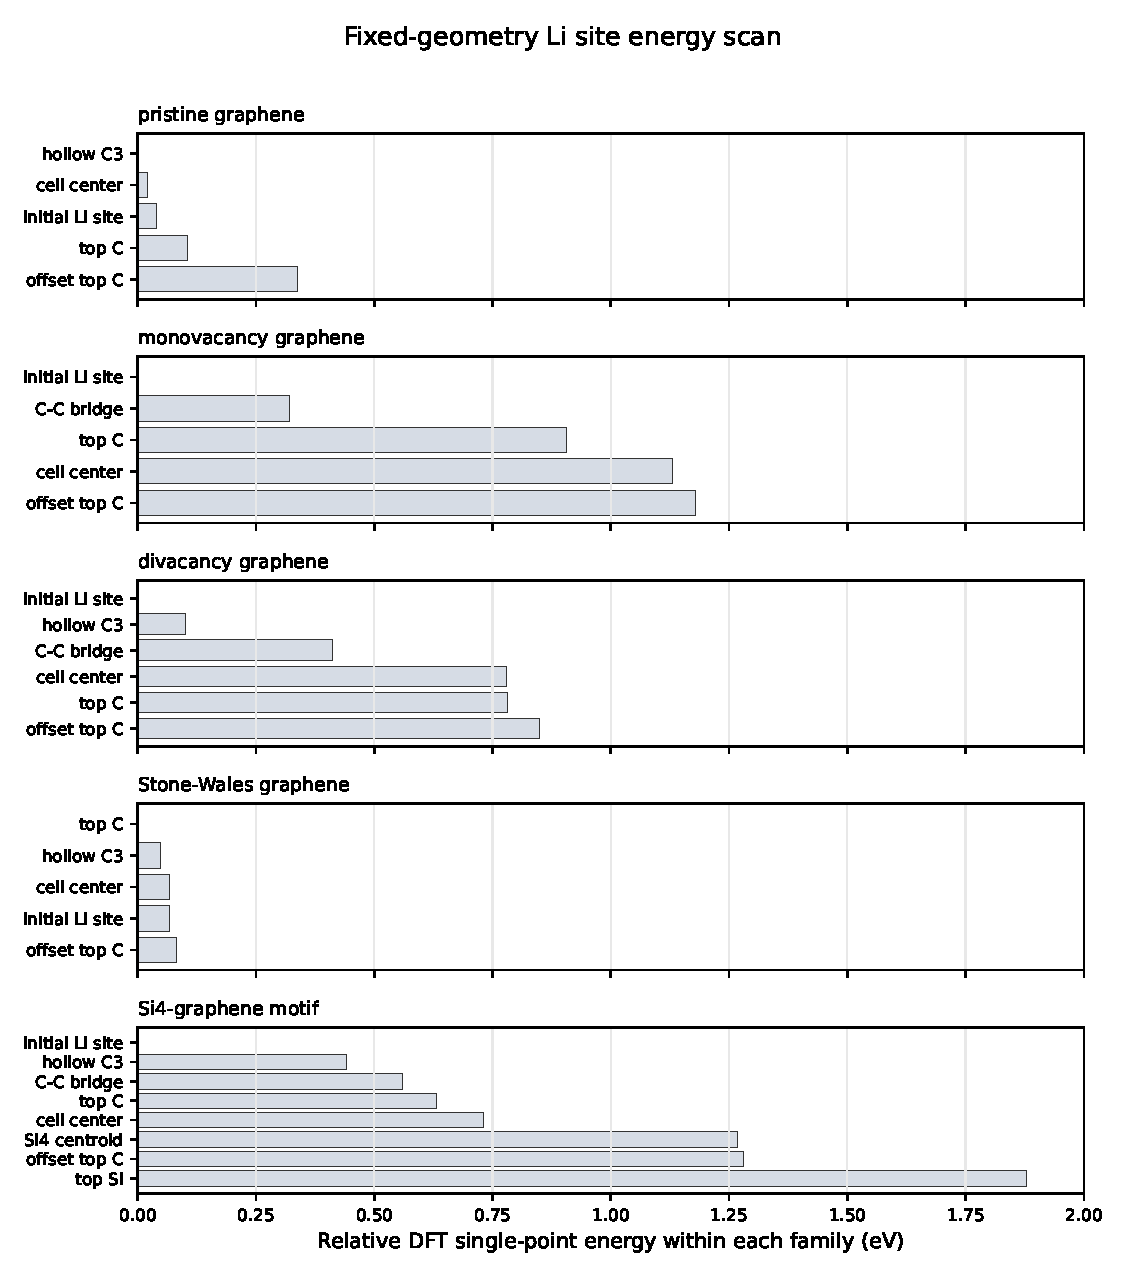
\includegraphics[width=0.88\textwidth]{site_energy_rankings_revised.pdf}
  \caption{DFT fixed-geometry Li site-energy scan. Each row is referenced to the
  lowest sampled site within the same structural family.}
  \label{fig:si_site_scan}
\end{figure}

\begin{figure}[H]
  \centering
  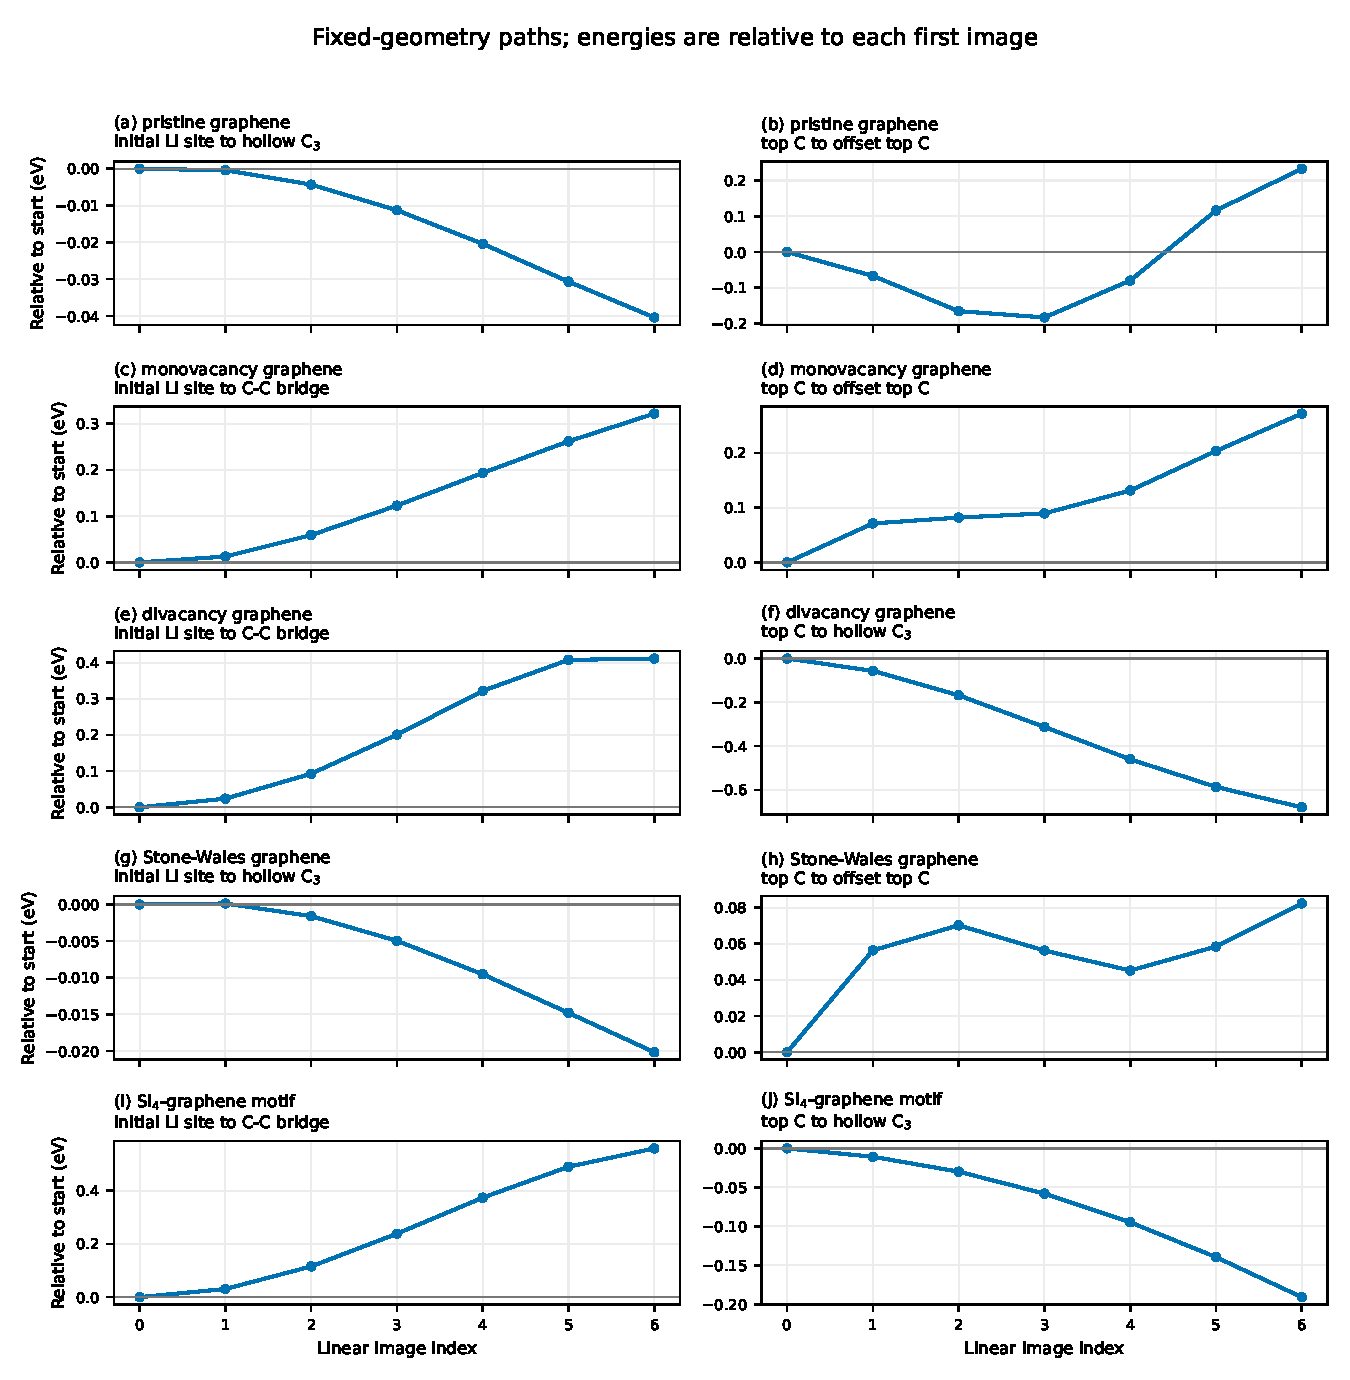
\includegraphics[width=0.75\textwidth]{path_profiles_revised.pdf}
  \caption{DFT fixed-geometry linear interpolation paths. Energies are
  referenced to the first image of each path. These profiles are configuration
  descriptors and are not minimum-energy paths.}
  \label{fig:si_path_scan}
\end{figure}

\begin{table}[H]
  \centering
  \footnotesize
  \caption{Fixed-geometry path descriptors. Path span is the maximum minus
  minimum single-point energy among the sampled interpolation images.}
  \label{tab:si_path_scans}
  \begin{tabular}{llcc}
    \toprule
    System & Path & Span (eV) & $\Delta E_{\mathrm{end-start}}$ (eV) \\
    \midrule
    Pristine & initial Li $\rightarrow$ hollow C$_3$ & 0.040 & -0.040 \\
    Pristine & top C $\rightarrow$ offset top C & 0.416 & 0.233 \\
    Monovacancy & initial Li $\rightarrow$ C--C bridge & 0.322 & 0.322 \\
    Monovacancy & top C $\rightarrow$ offset top C & 0.272 & 0.272 \\
    Divacancy & initial Li $\rightarrow$ C--C bridge & 0.411 & 0.411 \\
    Divacancy & top C $\rightarrow$ hollow C$_3$ & 0.680 & -0.680 \\
    Stone--Wales & initial Li $\rightarrow$ hollow C$_3$ & 0.020 & -0.020 \\
    Stone--Wales & top C $\rightarrow$ offset top C & 0.082 & 0.082 \\
    Si$_4$--graphene & initial Li $\rightarrow$ C--C bridge & 0.559 & 0.559 \\
    Si$_4$--graphene & top C $\rightarrow$ hollow C$_3$ & 0.191 & -0.191 \\
    \bottomrule
  \end{tabular}
\end{table}

\clearpage
\section{Finite-temperature trajectory context}

The finite-temperature trajectories were used to generate displaced
configurations for DFT force testing. The short and seed-sensitive traces are
not used to determine diffusion coefficients.

\begin{figure}[H]
  \centering
  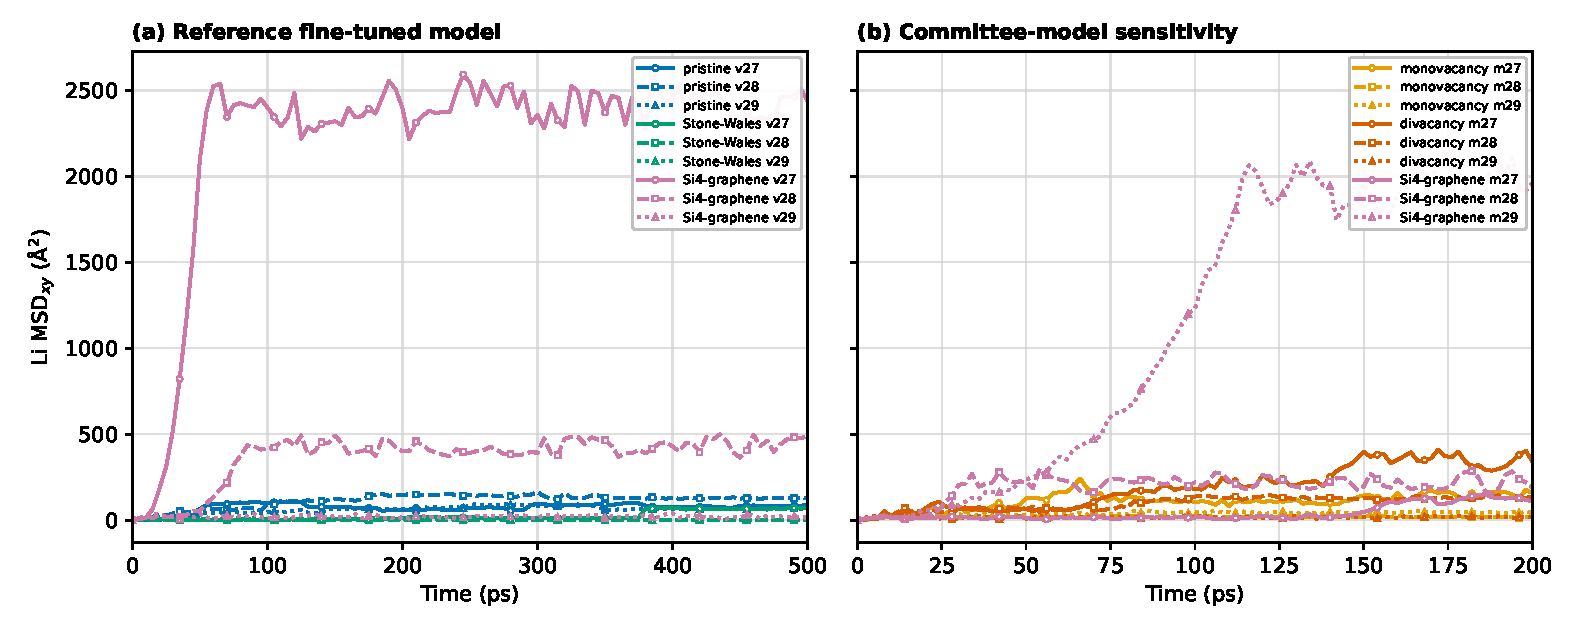
\includegraphics[width=\textwidth]{review_md_extended_msd_xy_traces.pdf}
  \caption{Unwrapped-coordinate Li in-plane MSD traces at 400 K. The left panel
  shows 500 ps reference-model trajectories and the right panel shows 200 ps
  committee-model trajectories. Labels v27--v29 and m27--m29 identify velocity
  and model seeds, respectively.}
  \label{fig:si_md_traces}
\end{figure}

\begin{table}[H]
  \centering
  \small
  \caption{Extended trajectory coverage and final in-plane MSD range.}
  \label{tab:si_md_runs}
  \begin{tabular}{llcc}
    \toprule
    System & Model set & Length (ps) & Final MSD$_{xy}$ (\AA$^2$) \\
    \midrule
    Pristine & Reference & 500 & 64.5--126.0 \\
    Monovacancy & Committee & 200 & 22.9--159.3 \\
    Divacancy & Committee & 200 & 16.0--341.1 \\
    Stone--Wales & Reference & 500 & 1.4--68.5 \\
    Si$_4$--graphene & Committee & 200 & 110.4--1963.4 \\
    Si$_4$--graphene & Reference & 500 & 13.6--2436.1 \\
    \bottomrule
  \end{tabular}
\end{table}

\clearpage
\section{DFT snapshot traceability}

All snapshots in Tables~\ref{tab:si_initial_snapshots} and
\ref{tab:si_extended_snapshots} reached electronic convergence and have
ASE-readable DFT forces. The versioned reproducibility archive records the input
provenance and OUTCAR SHA256 hash for every row.

\begin{table}[H]
  \centering
  \scriptsize
  \caption{Initial high-displacement snapshots used for direct MACE--DFT force
  comparisons. Energies are final VASP energies without entropy and serve as
  per-snapshot traceability values.}
  \label{tab:si_initial_snapshots}
  \begin{tabular}{llrrrp{3.4cm}}
    \toprule
    Case & seed/step & $t$ (ps) & MSD$_{xy}$ (\AA$^2$) & $E_{\mathrm{DFT}}$ (eV) & Shortest contacts (\AA) \\
    \midrule
    Si$_4$--graphene & 20260427/99700 & 99.7 & 2694.8 & -1898.927 & Li--C 2.19; Li--Si 2.60; Si--Si 2.09 \\
    Si$_4$--graphene & 20260427/99800 & 99.8 & 2683.4 & -1899.232 & Li--C 2.19; Li--Si 2.29; C--C 1.36 \\
    Si$_4$--graphene & 20260427/100000 & 100.0 & 2661.0 & -1902.314 & Li--C 2.10; Li--Si 2.35; C--C 1.36 \\
    Monovacancy & 20260429/58100 & 58.1 & 383.9 & -1407.426 & Li--C 1.91; C--C 1.20 \\
    Monovacancy & 20260429/58200 & 58.2 & 382.4 & -1407.643 & Li--C 1.92; C--C 1.21 \\
    Monovacancy & 20260429/100000 & 100.0 & 217.7 & -1406.797 & Li--C 1.85; C--C 1.22 \\
    Si$_4$--graphene & 20260429/30900 & 30.9 & 356.8 & -1897.170 & Li--C 2.19; Li--Si 2.57; Si--Si 2.15 \\
    Si$_4$--graphene & 20260429/31000 & 31.0 & 350.7 & -1899.553 & Li--C 2.13; Li--Si 2.49; Si--Si 1.99 \\
    Si$_4$--graphene & 20260429/100000 & 100.0 & 207.6 & -1902.948 & Li--C 2.24; Li--Si 2.66; Li--Li 3.73 \\
    \bottomrule
  \end{tabular}
\end{table}

\begin{table}[H]
  \centering
  \scriptsize
  \caption{Additional converged DFT checks from extended Si$_4$--graphene
  trajectories. These seven rows are not included in the nine-frame force RMSE
  comparison in the main text.}
  \label{tab:si_extended_snapshots}
  \begin{tabular}{llrrr}
    \toprule
    Model context & Velocity seed & $t$ (ps) & MSD$_{xy}$ (\AA$^2$) & $E_{\mathrm{DFT}}$ (eV) \\
    \midrule
    Reference fine-tuned & 20260427 & 57.0 & 2687.8 & -1899.725 \\
    Reference fine-tuned & 20260427 & 500.0 & 2436.1 & -1903.110 \\
    Committee seed 20260429 & 20260427 & 174.0 & 2167.7 & -1899.193 \\
    Committee seed 20260429 & 20260427 & 200.0 & 1963.4 & -1900.551 \\
    Reference fine-tuned & 20260428 & 423.0 & 525.1 & -1901.636 \\
    Reference fine-tuned & 20260428 & 496.0 & 527.1 & -1903.961 \\
    Reference fine-tuned & 20260428 & 500.0 & 489.5 & -1902.377 \\
    \bottomrule
  \end{tabular}
\end{table}

\end{document}
